\chapter{Handling data for training the model}\label{chapt:data}
\textit{As stated before in \cref{chapt:problem}, Images from Sentinel-2A have been used.}

\section{Get the raw training dataset}
Data needed for training the model is divided into two parts: \textbf{(a)} Satellite image and the \textbf{(b)} Labelled dataset of Roads. Both (a) and (b) should be from the same geography.

Satellite images for Sentinel-2A are available at \url{https://scihub.copernicus.eu/dhus/}. For deep learning, a very accurately labeled dataset is crucial for model training. The pixel-level dataset is challenging to produce in any small community. This is when the web-map services come into the picture. One of the popular mapping services is the Open Street Map~(OSM), which has been widely used to find the road vectors. I will use out satellite images with the road vectors obtained from OSM. An advantage of using OSM is that many human resources are saved, and the main work can be focussed on writing code to validate the research, thus making the process efficient.


\section{Converting data to a usable form}
Even after obtaining the satellite image and road dataset for the same geographical area, the final result image is quite big for Deep Convolutional Neural Network~(DCNN) to handle. To solve this problem, I sliced the image into multiple images of size $544\times544$ (\cref{fig:run_split_images}). This results in multiple small images which can be handled well by a computer (16~GB RAM). This size can be decreased or increased depending on the specifications of the computer used.
\begin{figure}[h!]
  \centering
  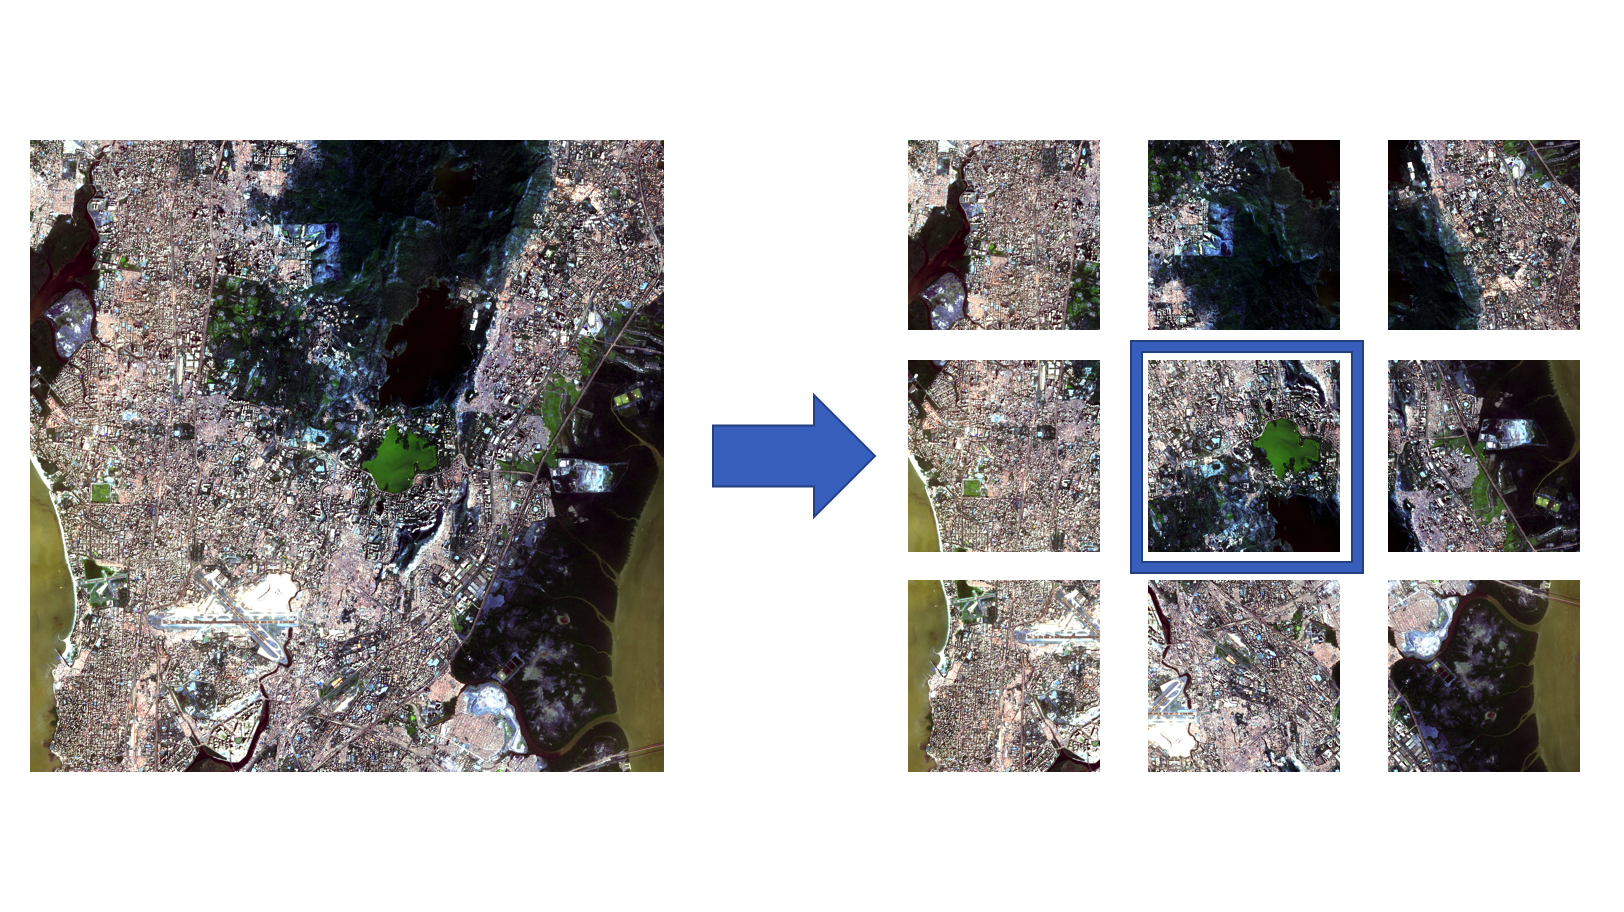
\includegraphics[width=\textwidth]{run_split_image}
  \caption{Image split into 9 parts making it fit for practical use in models.}
  \label{fig:run_split_images}
\end{figure}


\section{Cleaning the obtained dataset}
Though the data is from OSM by multiple collaborators, it is more or less in a raw format and prone to errors. Given its open-source in nature, it may be outdated or, in some cases, need some corrections. These corrections need to be manually done to ensure the training data is accurate before being fed into our model.

The images with less or no roads are removed from the dataset. This is so that `the no road` data should not affect the weights used to identify roads. This step is significant because roads often make up a tiny part of satellite images, and most training images will have no roads on them.


\section{Handling the noise generated to improve training}
Now that the models are chosen, we will now try to link the output of the super-resolution model to the input of road-detector. As specified earlier, our road-detection model assumes the training and input dataset ideally is a pixel-level accurate map. This is a problem as no super-resolution model can be 100 percent accurate. Thus, this underlying condition needs to be handled to reduce false predictions in the model.

The datasets constructed from a map suffers from two types of labeled noises (\cref{fig:noise_types}):
\begin{itemize}
  \setlength\itemsep{1pt}
  \item Omission noise is when the map is incomplete. It is true for small roads and alleys.
  \item Registration noise is when the location of the object is inaccurate. This noise is quite common, as maintaining pixel-level accuracy is quite difficult to produce.
\end{itemize}

\begin{figure}[h!]
  \centering
  \begin{subfigure}{0.63\textwidth}
    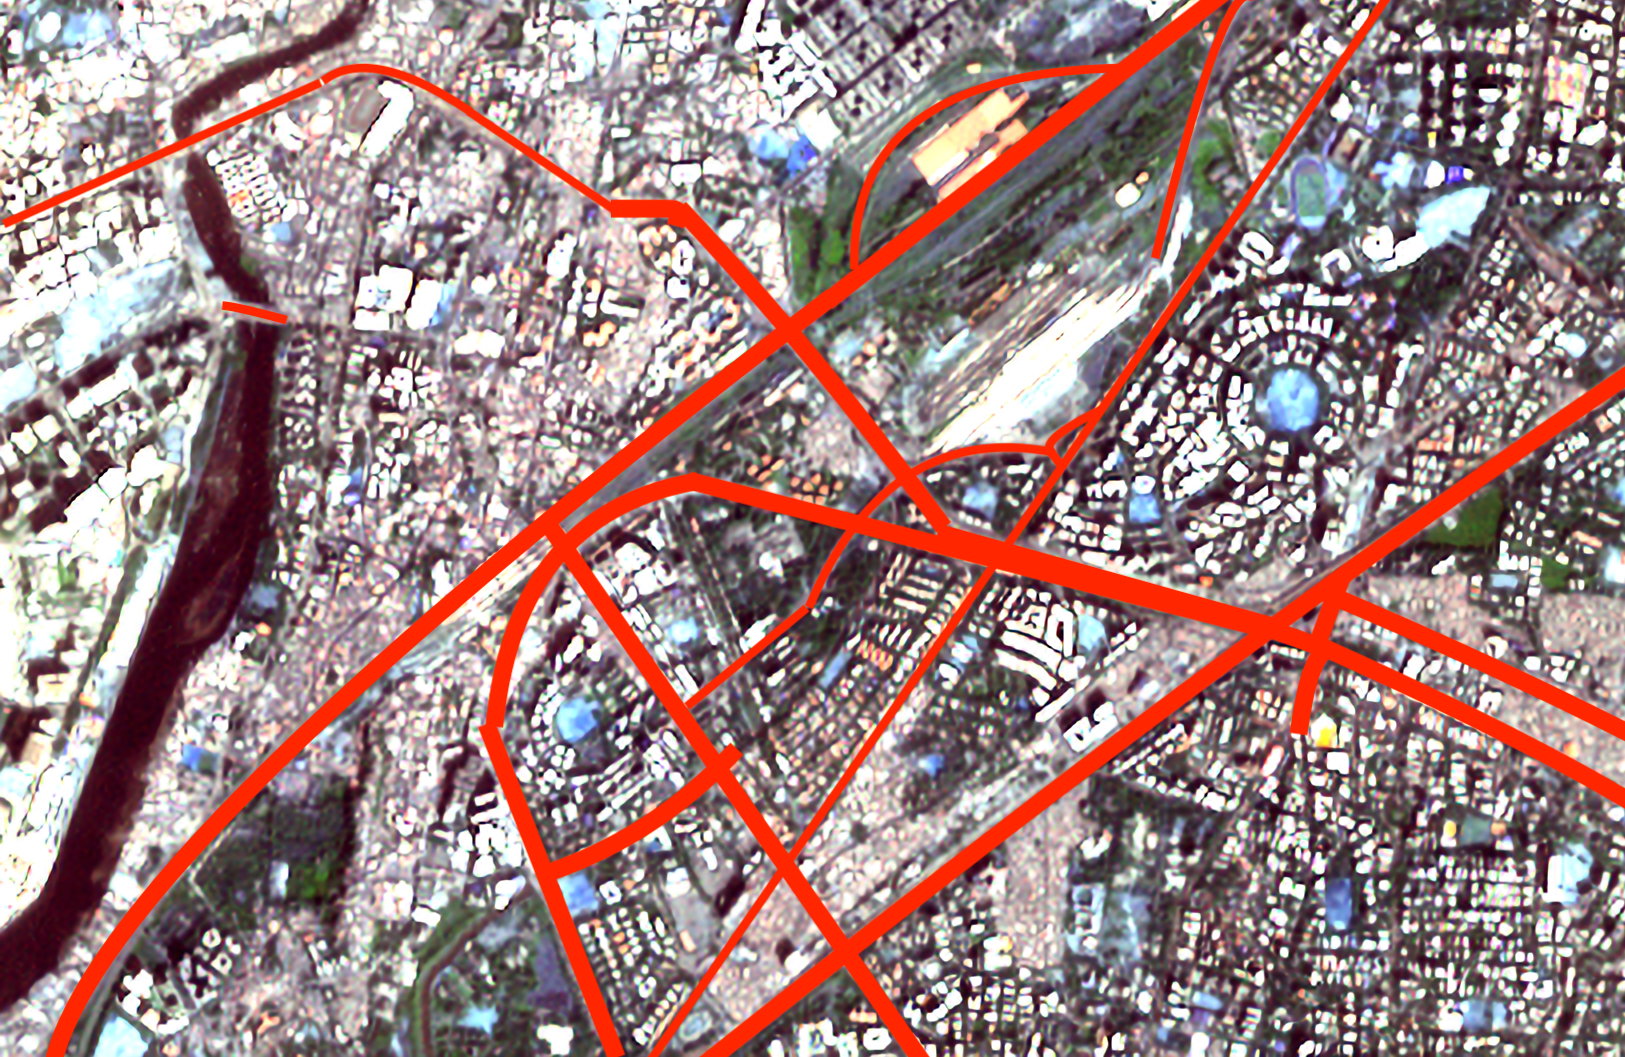
\includegraphics[width=\textwidth]{noise_omission}
    \caption{}
  \end{subfigure}~
  \begin{subfigure}{0.35\textwidth}
    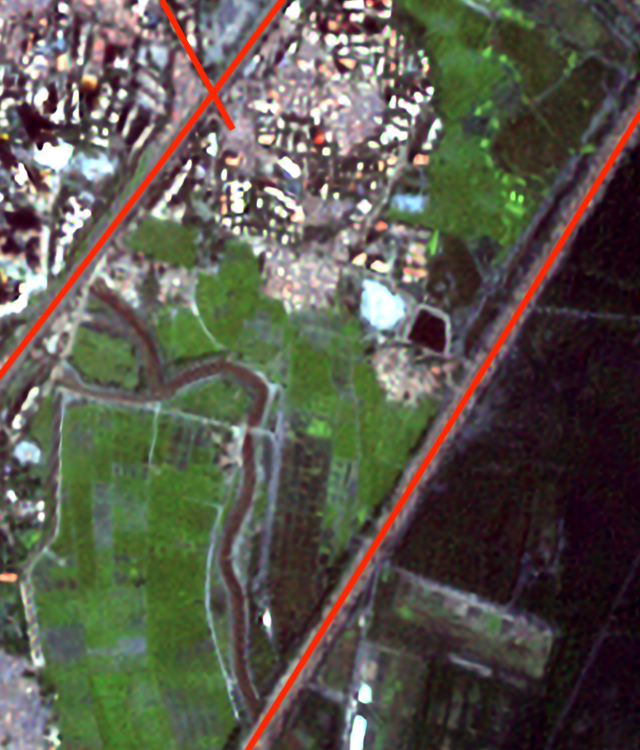
\includegraphics[width=\textwidth]{noise_registration}
    \caption{}
  \end{subfigure}
  \caption[Types of noises in a dataset]{Types of noises in a dataset \textbf{(a)}~Omission noise \textbf{(b)}~noise registration.}
  \label{fig:noise_types}
\end{figure}

These kinds of errors in the training labels reduce the accuracy of classifiers trained with this data. To solve this we use a proper loss function during training for our road-detection model.
